\documentclass[10pt,twocolumn]{article}

\usepackage[T1]{fontenc}
\usepackage{newtxtext}
\usepackage[margin=0.72in,columnsep=0.25in]{geometry}
\usepackage{microtype}
\usepackage{amsmath,amssymb,mathtools}
\usepackage{newtxmath}
\usepackage{booktabs,array,tabularx}
\usepackage{enumitem}
\usepackage{graphicx}
\usepackage{tikz}
\usetikzlibrary{arrows.meta,backgrounds,decorations.pathreplacing,fit}
\usepackage{xcolor}
\usepackage{caption}
\usepackage{subcaption}
\usepackage{placeins}
\usepackage[numbers,sort&compress]{natbib}
\usepackage{hyperref}
\usepackage{flushend}

\definecolor{accent}{HTML}{315A7D}
\definecolor{accentlight}{HTML}{EAF0F5}
\definecolor{grayfill}{HTML}{F3F3F3}
\definecolor{darkgray}{HTML}{4A4A4A}
\definecolor{mutedgreen}{HTML}{E5EFE7}

\hypersetup{
  colorlinks=true,
  linkcolor=accent,
  citecolor=accent,
  urlcolor=accent,
  pdftitle={Continuous Tokens: Lossless Latent Byte Spans for Vocabulary-Free Transformers},
  pdfauthor={Tamir Friedman, Daniel Alfasi, Netanel Moyal}
}

\captionsetup{font=small,labelfont=bf}
\setlist[itemize]{leftmargin=*,topsep=2pt,itemsep=1pt,parsep=0pt}
\setlist[enumerate]{leftmargin=*,topsep=2pt,itemsep=1pt,parsep=0pt}
\setlength{\parindent}{1em}
\setlength{\parskip}{0pt}
\setlength{\columnsep}{0.25in}
\renewcommand{\arraystretch}{1.12}

\pagestyle{plain}

\newcommand{\bytes}{\mathcal{B}}
\newcommand{\controls}{\mathcal{C}}
\newcommand{\reals}{\mathbb{R}}
\newcommand{\codeceos}{\textsc{CodecEos}}
\newcommand{\yes}{\textbf{Yes}}
\newcommand{\no}{No}

\tikzset{
  stage/.style={draw=black!65, line width=0.55pt, rounded corners=1.2pt, fill=grayfill,
    align=center, minimum height=8mm, text width=21mm, inner sep=2.5pt},
  neural/.style={stage, draw=accent, fill=accentlight},
  native/.style={stage, fill=white},
  data/.style={stage, rounded corners=0pt, fill=white, text width=18mm},
  flow/.style={-{Latex[length=1.8mm]}, line width=0.65pt, draw=black!75},
  feedback/.style={-{Latex[length=1.8mm]}, line width=0.65pt, draw=accent, dashed},
  region/.style={draw=black!55, line width=0.55pt, fill=grayfill, opacity=0.9},
  valid/.style={draw=black!60, fill=mutedgreen, rounded corners=1pt},
  invalid/.style={draw=black!45, fill=grayfill, rounded corners=1pt}
}

\title{\vspace{-0.48in}\textbf{Continuous Tokens: Lossless Latent Byte Spans\\
  for Vocabulary-Free Transformers}}
\author{
  Tamir Friedman$^{1,*}$ \quad Daniel Alfasi$^1$ \quad Netanel Moyal$^1$\\[2pt]
  \small $^1$Reco\\[-1pt]
  \small \href{mailto:tamirf@reco.ai}{\texttt{tamirf@reco.ai}} \quad
  \href{mailto:daniela@reco.ai}{\texttt{daniela@reco.ai}} \quad
  \href{mailto:netanelm@reco.ai}{\texttt{netanelm@reco.ai}}\\[-1pt]
  \small $^*$Corresponding author
}
\date{\small August 2026}

\begin{document}
\maketitle
\thispagestyle{plain}

\begin{abstract}
Subword tokenization maps byte strings to discrete identifiers and then maps those identifiers to
rows in large embedding and output matrices. We ask whether the identifier and the ordinary
vocabulary are necessary at all. A \emph{continuous token} is a non-empty variable-length byte
span represented directly by a generated latent vector. A small local decoder certifies the exact
payload by reconstructing the bytes and a private end marker; a one-byte path is always an exact
fallback. The idea is deliberately modular. An input-only tokenizer can replace ordinary input
lookup while preserving a frozen language-model backbone and native output head. An output-only
tokenizer can map frozen hidden states to byte spans while retaining native input feedback. When
composed, generated bytes are fed directly through the continuous input tokenizer, eliminating
ordinary token IDs, the subword embedding table, and the vocabulary-sized output projection.
Only byte primitives and a small structural-control interface remain discrete. We formalize the
protocol, describe a compatibility bridge for existing models, derive its potential memory and
compute advantages, and specify experiments that can falsify the proposal. Preliminary observations
demonstrate native-head bypass and multi-byte macro-steps, but do not yet establish exact output
generation or behavioral equivalence. We therefore present a modular architecture, analytical
hypotheses, and a prospective empirical program rather than a claim of completed validation.
\end{abstract}

\noindent\textbf{Keywords:} tokenization, byte models, latent representations, sequence
compression, language models.

\section{Introduction}

Transformers process vectors \citep{vaswani2017attention}, yet most language-model interfaces
insist on an intermediate discrete subword identity. A tokenizer first partitions text into
members of a fixed vocabulary;
an embedding table then turns each identity back into a vector. Generation reverses the pattern:
a vocabulary-sized projection scores identities, which are finally decoded to bytes. This design
is effective, but the global model inherits the vocabulary's fixed boundaries, parameter cost,
language bias, and update cycle.

Byte-level models remove the vocabulary but increase the number of global positions. Patch and
character models reduce that cost by pooling local symbols, but their latent units are generally
internal, contextual, or not independently reversible. We explore a third point in the design
space: a local neural tokenizer that maps an arbitrary candidate byte span to one continuous
latent and accepts it only when a deterministic local decoder recovers the exact bytes.

The proposal has three deployment forms, illustrated in Figure~\ref{fig:architecture}:

\begin{itemize}
  \item \textbf{Input-only:} replace ordinary input tokenization and lookup; retain the frozen
  backbone, native output head, native output tokenizer, and structural controls.
  \item \textbf{Output-only:} decode frozen final hidden states to non-empty byte spans or
  controls; retain the native input path for feedback.
  \item \textbf{Combined input-output:} compose both directions, feed generated bytes back through
  the continuous input tokenizer, and remove both ordinary vocabulary matrices.
\end{itemize}

Modularity is an advantage rather than a concession. Each direction can be tested, deployed, and
rolled back independently. The combined system is the architectural end-state; the directional
systems are useful products and controlled scientific ablations in their own right.

Our contributions are:

\begin{enumerate}
  \item a codebook-free definition of a lossless continuous byte-span token;
  \item an exhaustive segmentation rule that remains correct under non-monotonic validity;
  \item modular input-only, output-only, and combined input-output Transformer interfaces;
  \item a compatibility curriculum that intentionally overfits a frozen native embedding table;
  \item an analytical account of vocabulary-state, KV-cache, context, and compute savings; and
  \item a falsifiable evaluation protocol that separates exactness, behavior, density, and systems
  performance.
\end{enumerate}

\section{Background and Related Work}

BPE and related subword methods address open-vocabulary language by composing frequent discrete
units~\citep{sennrich2016bpe}. SentencePiece makes subword training language-independent and works
directly from raw sentences~\citep{kudo2018sentencepiece}. These methods remain vocabulary based:
each global position selects one row from a finite table.

Token-free models instead expose small alphabets to the network. ByT5 processes UTF-8 bytes and
demonstrates robustness without a text tokenizer~\citep{xue2022byt5}; CANINE operates directly on
characters while using downsampling for efficiency~\citep{clark2022canine}. Their challenge is
sequence expansion: a word represented by several bytes consumes several global positions.
Charformer learns differentiable subword blocks through gradient-based tokenization
\citep{tay2022charformer}. BLT dynamically groups bytes into patches and allocates large-model
computation according to local entropy~\citep{pagnoni2024blt}. These systems establish that local
byte or character computation can support stronger global units.

Our proposal differs in two coupled requirements. First, a span is accepted only after exact,
independent round-trip reconstruction. Second, the global unit is continuous and has no codebook
identifier. VQ-VAE demonstrates the usefulness of learned discrete latent codes
\citep{oord2017vqvae}; continuous tokens deliberately omit that quantization. The output Transformer
need only produce a latent inside the decoder region corresponding to the desired byte span, not a
particular codebook entry.

\begin{table}[t]
\centering
\caption{Positioning within the tokenization design space. ``Independent inverse'' means that one
global unit can be decoded to its exact local payload without the original input sequence.}
\label{tab:related}
\scriptsize
\begin{tabularx}{\columnwidth}{@{}l >{\raggedright\arraybackslash}X c c c@{}}
\toprule
Method & Global unit & Fixed $V$ & Exact & Retrofit \\
\midrule
BPE / SentencePiece & token ID & \yes & \yes & \yes \\
ByT5 / CANINE & byte / character & \no & Trivial & \no \\
Charformer & learned block & \no & \no & \no \\
BLT & contextual patch & \no & \no & \no \\
Continuous tokens & latent vector & \no & \yes & \yes \\
\bottomrule
\end{tabularx}
\end{table}

\section{Continuous Token Protocol}

Let the byte alphabet be $\bytes=\{0,\ldots,255\}$ and let $\controls$ be a small set of model
protocol controls such as beginning-of-sequence, end-of-sequence, and role markers. Controls are
structural events, not byte spellings. They bypass the byte tokenizer and preserve their exact
semantics.

\subsection{A reversible latent span}

For a maximum local span length $L$, the input byte-span codec contains
\begin{align}
E_\theta &: \bytes^{1:L} \rightarrow \reals^d, \\
D_\phi &: \reals^d \rightarrow (\bytes \cup \{\codeceos\})^{L+1}.
\end{align}
The decoder is parallel: learned output-position queries attend to one latent memory vector and
produce 257-way logits. Greedy decoding terminates at the first private $\codeceos$. This symbol
belongs only to the local codec; it has no input embedding and is unrelated to the language
model's structural end-of-sequence control.

A candidate span $s$ is valid exactly when
\begin{equation}
\operatorname{valid}(s) \iff D_{\phi,0}(E_\theta(s)) = s\,\Vert\,\codeceos,
\label{eq:valid}
\end{equation}
including the termination position. Every atomic byte bypasses the learned composition path and
uses its exact frozen byte embedding. Atomic spans are therefore total, deterministic fallbacks.

The decoder partitions continuous space into implicit regions
\begin{equation}
\mathcal{R}_s = \{z \in \reals^d : D_{\phi,0}(z)=s\,\Vert\,\codeceos\}.
\end{equation}
There is no discrete codebook. For input, $E_\theta(s)$ must land inside $\mathcal{R}_s$. For
output, a hidden-state adapter needs only to land anywhere inside the same region. Noise and margin
training can enlarge useful regions around canonical encoder outputs.

\subsection{Exhaustive non-monotonic segmentation}

Validity need not be monotonic in span length: a four-byte candidate may fail while a five-byte
candidate succeeds. Consequently, a failure must never prune longer candidates. At byte offset
$i$, all lengths are encoded and decoded in one padded batch, and the tokenizer selects
\begin{equation}
\ell_i^* = \max\left(\{1\}\cup
\left\{\ell\in[2,L] : \operatorname{valid}(x_{i:i+\ell})\right\}\right).
\label{eq:segment}
\end{equation}
The default objective is longest-valid greedy segmentation. Dynamic programming can later replace
the local objective without changing the codec protocol.

An encoding-only LRU cache may memoize $s\mapsto E_\theta(s)$ when evaluation is deterministic.
It must return a bit-identical CPU copy, must not cache validity, and must never change candidate
enumeration or acceptance. In the limit, a frozen cache of known spans behaves like a conventional
embedding vocabulary, while the neural path supplies an open long tail.

\begin{figure*}[t]
\centering
\begin{subfigure}[t]{0.49\textwidth}
\centering
\resizebox{\linewidth}{!}{%
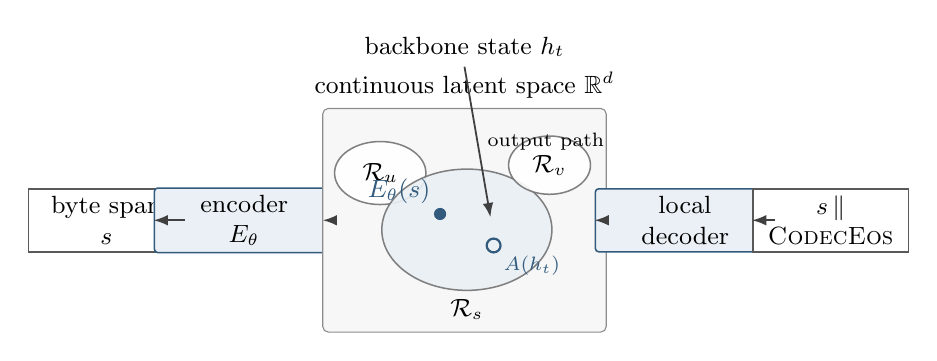
\begin{tikzpicture}[font=\small]
  \node[data] (span) at (0,0) {byte span\\$s$};
  \node[neural] (enc) at (1.75,0) {encoder\\$E_\theta$};
  \draw[flow] (span) -- (enc);

  \draw[draw=black!45, rounded corners=2pt, fill=grayfill!65]
    (2.75,-1.42) rectangle (6.35,1.42);
  \node[font=\small, anchor=south] at (4.55,1.42) {continuous latent space $\reals^d$};
  \draw[region, fill=white] (3.48,0.60) ellipse (0.58 and 0.40);
  \draw[region, fill=accentlight] (4.58,-0.12) ellipse (1.08 and 0.77);
  \draw[region, fill=white] (5.63,0.70) ellipse (0.52 and 0.37);
  \node[font=\small] at (3.48,0.60) {$\mathcal{R}_{u}$};
  \node[font=\small, anchor=north] at (4.58,-0.88) {$\mathcal{R}_{s}$};
  \node[font=\small] at (5.63,0.70) {$\mathcal{R}_{v}$};
  \fill[accent] (4.24,0.08) circle (2.2pt) node[above left, font=\small] {$E_\theta(s)$};
  \draw[accent, line width=0.8pt] (4.92,-0.32) circle (2.5pt)
    node[below right, font=\scriptsize] {$A(h_t)$};
  \draw[flow] (enc.east) -- (2.75,0);
  \draw[flow] (4.55,1.95) -- node[right, font=\scriptsize] {output path} (4.88,0.04);
  \node[above, font=\small] at (4.55,1.95) {backbone state $h_t$};

  \node[neural] (dec) at (7.35,0) {local\\decoder};
  \node[data] (decoded) at (9.20,0) {$s\,\Vert$\\$\codeceos$};
  \draw[flow] (6.35,0) -- (dec);
  \draw[flow] (dec) -- (decoded);
\end{tikzpicture}}
\caption{The decoder induces regions in continuous space. The input encoding $E_\theta(s)$ and an
output adapter value $A(h_t)$ may differ numerically while decoding to the same exact span $s$.}
\label{fig:regions}
\end{subfigure}\hfill
\begin{subfigure}[t]{0.49\textwidth}
\centering
\resizebox{\linewidth}{!}{%
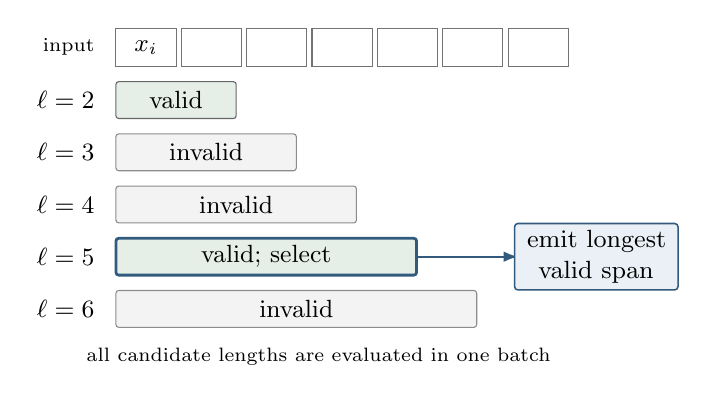
\begin{tikzpicture}[font=\small, x=0.83cm, y=0.78cm]
  \foreach \x/\label in {0/$x_i$,1/{},2/{},3/{},4/{},5/{},6/{}} {
    \draw[fill=white, draw=black!55] (\x,1.10) rectangle +(0.92,0.62);
    \node at (\x+0.46,1.41) {\label};
  }
  \node[anchor=east, font=\scriptsize] at (-0.18,1.41) {input};

  \node[anchor=east] at (-0.18,0.55) {$\ell=2$};
  \draw[valid] (0,0.25) rectangle (1.84,0.85);
  \node at (0.92,0.55) {valid};

  \node[anchor=east] at (-0.18,-0.30) {$\ell=3$};
  \draw[invalid] (0,-0.60) rectangle (2.76,0);
  \node at (1.38,-0.30) {invalid};

  \node[anchor=east] at (-0.18,-1.15) {$\ell=4$};
  \draw[invalid] (0,-1.45) rectangle (3.68,-0.85);
  \node at (1.84,-1.15) {invalid};

  \node[anchor=east] at (-0.18,-2.00) {$\ell=5$};
  \draw[valid, draw=accent, line width=1.0pt] (0,-2.30) rectangle (4.60,-1.70);
  \node at (2.30,-2.00) {valid; select};

  \node[anchor=east] at (-0.18,-2.85) {$\ell=6$};
  \draw[invalid] (0,-3.15) rectangle (5.52,-2.55);
  \node at (2.76,-2.85) {invalid};

  \draw[flow, draw=accent] (4.60,-2.00) -- (6.15,-2.00);
  \node[neural, text width=19mm] at (7.35,-2.00) {emit longest\\valid span};
  \node[font=\scriptsize, align=center] at (3.10,-3.62)
    {all candidate lengths are evaluated in one batch};
\end{tikzpicture}}
\caption{Validity is non-monotonic. Failure at lengths three and four does not prune the valid
length-five candidate. If every multi-byte candidate fails, the exact atomic-byte path is used.}
\label{fig:nonmonotonic}
\end{subfigure}
\caption{Two mechanics of continuous byte-span tokenization: codebook-free latent decoding regions
and exhaustive longest-valid segmentation.}
\label{fig:mechanics}
\end{figure*}

\begin{figure*}[t]
\centering
\resizebox{0.96\textwidth}{!}{%
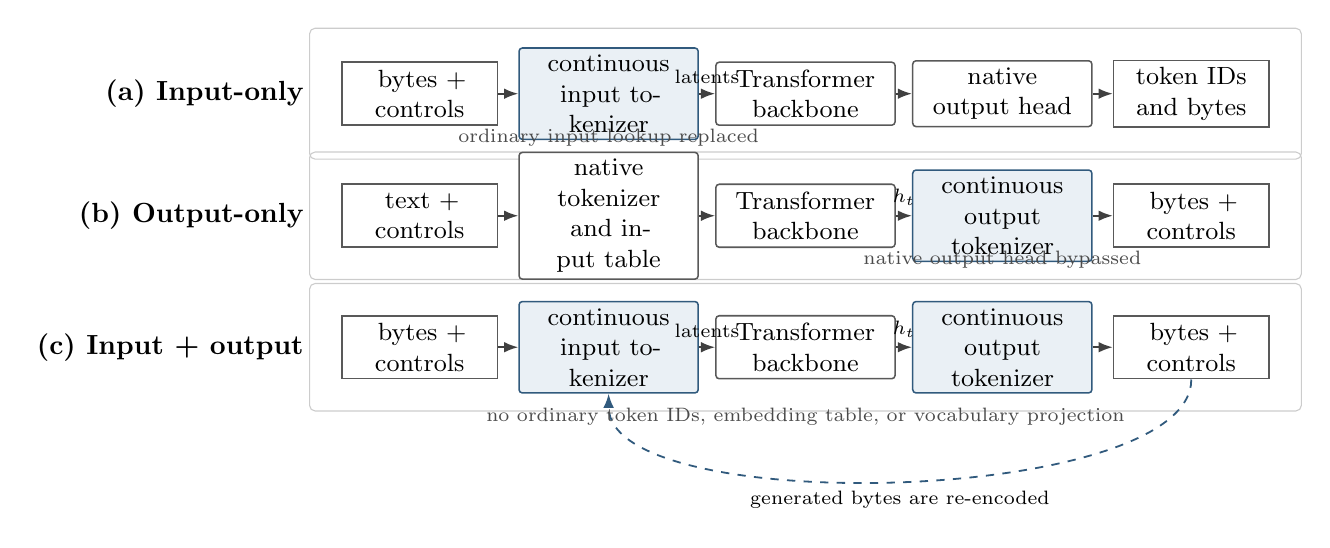
\begin{tikzpicture}[font=\small]
  \node[anchor=east, font=\bfseries] at (-0.35,0) {(a) Input-only};
  \node[data]   (i-data) at (1.0,0) {bytes +\\controls};
  \node[neural] (i-in)   at (3.4,0) {continuous\\input tokenizer};
  \node[native] (i-lm)   at (5.9,0) {Transformer\\backbone};
  \node[native] (i-head) at (8.4,0) {native\\output head};
  \node[data]   (i-out)  at (10.8,0) {token IDs\\and bytes};
  \draw[flow] (i-data) -- (i-in);
  \draw[flow] (i-in) -- node[above, font=\scriptsize]{latents} (i-lm);
  \draw[flow] (i-lm) -- (i-head);
  \draw[flow] (i-head) -- (i-out);
  \node[font=\scriptsize, text=darkgray] at (3.4,-0.56) {ordinary input lookup replaced};

  \node[anchor=east, font=\bfseries] at (-0.35,-1.55) {(b) Output-only};
  \node[data]   (o-data) at (1.0,-1.55) {text +\\controls};
  \node[native] (o-in)   at (3.4,-1.55) {native tokenizer\\and input table};
  \node[native] (o-lm)   at (5.9,-1.55) {Transformer\\backbone};
  \node[neural] (o-out)  at (8.4,-1.55) {continuous\\output tokenizer};
  \node[data]   (o-data2) at (10.8,-1.55) {bytes +\\controls};
  \draw[flow] (o-data) -- (o-in);
  \draw[flow] (o-in) -- (o-lm);
  \draw[flow] (o-lm) -- node[above, font=\scriptsize]{$h_t$} (o-out);
  \draw[flow] (o-out) -- (o-data2);
  \node[font=\scriptsize, text=darkgray] at (8.4,-2.11) {native output head bypassed};

  \node[anchor=east, font=\bfseries] at (-0.35,-3.22) {(c) Input + output};
  \node[data]   (c-data) at (1.0,-3.22) {bytes +\\controls};
  \node[neural] (c-in)   at (3.4,-3.22) {continuous\\input tokenizer};
  \node[native] (c-lm)   at (5.9,-3.22) {Transformer\\backbone};
  \node[neural] (c-out)  at (8.4,-3.22) {continuous\\output tokenizer};
  \node[data]   (c-data2) at (10.8,-3.22) {bytes +\\controls};
  \draw[flow] (c-data) -- (c-in);
  \draw[flow] (c-in) -- node[above, font=\scriptsize]{latents} (c-lm);
  \draw[flow] (c-lm) -- node[above, font=\scriptsize]{$h_t$} (c-out);
  \draw[flow] (c-out) -- (c-data2);
  \draw[feedback] (c-data2.south) to[out=-90,in=-90,looseness=0.55]
    node[below, font=\scriptsize]{generated bytes are re-encoded} (c-in.south);
  \node[font=\scriptsize, text=darkgray] at (5.9,-4.10)
    {no ordinary token IDs, embedding table, or vocabulary projection};

  \begin{scope}[on background layer]
    \node[fit=(i-data)(i-out), draw=black!20, rounded corners=2pt, inner sep=4mm] {};
    \node[fit=(o-data)(o-data2), draw=black!20, rounded corners=2pt, inner sep=4mm] {};
    \node[fit=(c-data)(c-data2), draw=black!20, rounded corners=2pt, inner sep=4mm] {};
  \end{scope}
\end{tikzpicture}
}
\caption{Three deployment forms of the same modular idea. Light blue boxes are learned continuous
tokenizers; white boxes are retained native components. Input-only and output-only can be evaluated
or deployed independently. Their composition closes the byte feedback loop and removes ordinary
token IDs and both vocabulary-sized interfaces. Structural controls bypass the byte path.}
\label{fig:architecture}
\end{figure*}
\FloatBarrier

\section{Three Modular Deployment Forms}

\subsection{Input-only replacement}

Let $W_{\mathrm{in}}\in\reals^{V\times d}$ be a frozen native input table. For an ordinary native
token $v$ with canonical byte payload $s_v$, define its compatibility target by
\begin{equation}
E_\theta(s_v) \approx W_{\mathrm{in}}[v].
\end{equation}
Compatibility mode preserves native boundaries and changes only how ordinary embeddings are
produced. Structural controls use their exact frozen rows. Dense mode then merges neighboring
bytes whenever Equation~\ref{eq:valid} succeeds. The backbone consumes the resulting sequence via
its ordinary continuous embedding interface.

This module is useful by itself: denser prompts can reduce global positions, KV-cache state, and
prefill work while the native output distribution remains untouched. An untied input table can be
physically omitted after replacement. A tied input/output table cannot be removed while the native
output head still depends on it; that is an applicability limit, not a failure of input density.

\subsection{Output-only generation}

An output tokenizer maps the final hidden state $h_t$ to either a structural control or a non-empty
byte span. A parallel byte decoder predicts a finite sequence ending in its private termination
symbol. In the standalone output-only form, emitted bytes are deterministically segmented into
native token IDs for feedback to the unchanged input path. This permits a controlled experiment:
the backbone and native feedback remain fixed while the vocabulary-sized output head is bypassed.

The output module can produce several bytes per global macro-step. Its central learning challenge
is not reconstruction but conditional prediction: a long span must be both decodable and
predictable from $h_t$. Sampling must also remain meaningful when probabilities are defined over
byte positions rather than a flat token vocabulary.

\subsection{Combined input-output replacement}

In the combined system, emitted bytes return through the continuous input tokenizer. The feedback
loop contains no ordinary native token IDs. Structural controls remain explicit and small;
ordinary language, programming-language text, binary content, and all text encodings share the
same byte path.

This composition removes the ordinary input embedding matrix and the vocabulary-sized output
projection, including the single shared matrix in a tied model. The global interface becomes
conceptually smaller:
\begin{equation*}
\begin{aligned}
\text{bytes} &\rightarrow \text{local latent spans} \rightarrow \text{backbone}\\
&\rightarrow \text{local byte spans}.
\end{aligned}
\end{equation*}
The claim is not that the complete network has no interface cost. It retains 256 byte primitives,
structural controls, and local neural modules. The claim is that interface state and decisions no
longer scale with an arbitrary vocabulary size $V$.

\section{Training Strategy}

\subsection{Input curriculum}

The native table is a finite supervised data set. Let $z_v=E_\theta(s_v)$. Stage 1 intentionally
overfits every reachable, unambiguous ordinary row with
\begin{equation}
\begin{aligned}
\mathcal{L}_{\mathrm{in}} ={}&
\lambda_a\frac{\|z_v-W_{\mathrm{in}}[v]\|_2^2}
{\|W_{\mathrm{in}}[v]\|_2^2+\epsilon}\\
&+\lambda_r\operatorname{CE}\!\left(D_\phi(z_v),s_v\Vert\codeceos\right).
\end{aligned}
\label{eq:inputloss}
\end{equation}
The 256 atomic byte rows and control rows are copied and frozen. Duplicate native IDs that decode
to identical bytes but have different embeddings expose an information-theoretic conflict: one
deterministic byte mapping cannot equal two targets. Such aliases must be reported, canonicalized,
or retained structurally; they cannot be hidden by the loss.

Stage 2 freezes the selected aligned encoder and teaches its decoder arbitrary corpus and binary
spans, replaying vocabulary payloads to preserve exactness. Stage 3, when needed, freezes every
language-model parameter and distills native continuation behavior into dense input spans. Only
the input tokenizer receives gradients.

\subsection{Output curriculum}

The output tokenizer trains on frozen backbone hidden states paired with the next byte span or
control event. A practical curriculum begins with native-token payload boundaries, then grows to
multi-token and arbitrary byte spans. Exact termination, byte accuracy, and feedback equivalence
are optimized separately. Robustness noise around successful latent regions can make exact greedy
decoding less brittle.

For an output decoder $O_\psi$, a simplified objective is
\begin{equation}
\begin{aligned}
\mathcal{L}_{\mathrm{out}} =
{}&\operatorname{CE}\!\left(O_\psi(h_t),s_{t+1}\Vert\codeceos\right)\\
&+\lambda_f\mathcal{L}_{\mathrm{feedback}}
+\lambda_c\mathcal{L}_{\mathrm{control}}.
\end{aligned}
\end{equation}
In a frozen-backbone retrofit, only $\psi$ and any small hidden-to-latent adapter train. In a future
from-scratch model, both directional tokenizers and the backbone could be co-trained, but that is a
different empirical claim.

\subsection{Why the modules stay separable}

Input and output tokenizers share a byte protocol but optimize different conditional problems.
The input encoder compresses an observed span; the output decoder predicts an unobserved span.
Separate checkpoints and gates therefore improve clarity. They may share byte embeddings or local
features only after independent evidence shows that sharing helps rather than entangles the two
objectives.

\section{Potential Systems Advantages}

\subsection{Vocabulary state}

Let $p$ be bytes per parameter, $d$ the model width, and $V$ the ordinary vocabulary size. Native
interface state is approximately
\begin{equation}
M_{\mathrm{native}} =
\begin{cases}
pVd, & \text{tied input/output matrix},\\
2pVd, & \text{untied matrices}.
\end{cases}
\end{equation}
The combined interface instead requires
\begin{equation}
M_{\mathrm{continuous}} \approx pP_{\mathrm{local}} + p(256+|\controls|)d,
\end{equation}
where $P_{\mathrm{local}}$ counts input and output tokenizer parameters. The proposal saves memory
only when the full deployed local state is smaller than the removed matrix state. Table
\ref{tab:state} gives illustrative BF16 arithmetic before local-module cost; these are not measured
model results.

\begin{table}[t]
\centering
\caption{Illustrative BF16 matrix state. ``Byte rows'' counts 256 model-width rows and excludes the
local neural modules. MiB uses $2^{20}$ bytes.}
\label{tab:state}
\small
\begin{tabular}{@{}r r r r@{}}
\toprule
$V$ & $d$ & One $V\!\times\!d$ matrix & 256 byte rows \\
\midrule
50,000  & 768   & 73.2 MiB  & 0.38 MiB \\
128,000 & 4,096 & 1,000 MiB & 2.00 MiB \\
250,000 & 1,024 & 488.3 MiB & 0.50 MiB \\
\bottomrule
\end{tabular}
\end{table}

\subsection{Positions, KV cache, and context}

Let $\rho$ be the ratio of native positions to continuous positions for identical bytes. If
$\rho>1$, a prompt requiring $T$ native positions requires approximately $T/\rho$ continuous
positions. KV-cache state is linear in global positions,
\begin{equation}
M_{\mathrm{KV}} \propto T\,N_{\mathrm{layers}}\,N_{\mathrm{kv}}\,d_h\,p,
\end{equation}
so the idealized KV ratio is $1/\rho$. At fixed global context length, byte capacity grows by
$\rho$. Dense prefill attention scales approximately as $1/\rho^2$ and per-position feed-forward
work as $1/\rho$, before local-tokenizer overhead.

\begin{table}[t]
\centering
\caption{Idealized global-work ratios for density $\rho$. Local tokenizer work, padding, kernels,
and hardware utilization are excluded and must be measured end to end.}
\label{tab:density}
\scriptsize
\begin{tabular}{@{}c c c c@{}}
\toprule
$\rho$ & KV / FFN & Attention & Context gain \\
\midrule
1.25 & 0.80 & 0.64 & 1.25$\times$ \\
1.50 & 0.67 & 0.44 & 1.50$\times$ \\
2.00 & 0.50 & 0.25 & 2.00$\times$ \\
3.00 & 0.33 & 0.11 & 3.00$\times$ \\
\bottomrule
\end{tabular}
\end{table}

The local codec is not free. Candidate enumeration, exact decoding, and output-span generation can
erase theoretical savings if implemented poorly. Batched candidates, bounded span lengths,
source-dtype deployment, model-local compilation, and encoding memoization are engineering tools,
not substitutes for end-to-end measurements.

\begin{figure*}[t]
\centering
\begin{subfigure}[t]{0.49\textwidth}
\centering
\resizebox{\linewidth}{!}{%
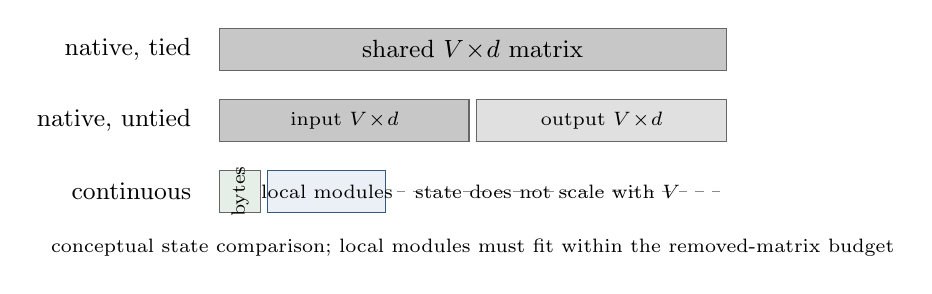
\begin{tikzpicture}[font=\small, x=0.92cm, y=0.82cm]
  \node[anchor=east] at (0,1.45) {native, tied};
  \draw[fill=black!22, draw=black!60] (0.25,1.12) rectangle (7.25,1.78);
  \node at (3.75,1.45) {shared $V\!\times\!d$ matrix};

  \node[anchor=east] at (0,0.35) {native, untied};
  \draw[fill=black!22, draw=black!60] (0.25,0.02) rectangle (3.70,0.68);
  \draw[fill=black!12, draw=black!60] (3.80,0.02) rectangle (7.25,0.68);
  \node[font=\scriptsize] at (1.98,0.35) {input $V\!\times\!d$};
  \node[font=\scriptsize] at (5.53,0.35) {output $V\!\times\!d$};

  \node[anchor=east] at (0,-0.75) {continuous};
  \draw[fill=mutedgreen, draw=black!60] (0.25,-1.08) rectangle (0.82,-0.42);
  \draw[fill=accentlight, draw=accent] (0.92,-1.08) rectangle (2.55,-0.42);
  \node[font=\scriptsize, rotate=90] at (0.54,-0.75) {bytes};
  \node[font=\scriptsize] at (1.74,-0.75) {local modules};
  \draw[dashed, draw=black!45] (2.70,-0.75) -- (7.25,-0.75);
  \node[font=\scriptsize, anchor=west] at (2.82,-0.75) {state does not scale with $V$};

  \node[font=\scriptsize, align=center] at (3.75,-1.62)
    {conceptual state comparison; local modules must fit within the removed-matrix budget};
\end{tikzpicture}}
\caption{Ordinary native interface state scales with vocabulary size $V$. In the combined system,
only byte/control rows and local tokenizer parameters remain at the interface.}
\label{fig:statebars}
\end{subfigure}\hfill
\begin{subfigure}[t]{0.49\textwidth}
\centering
\resizebox{\linewidth}{!}{%
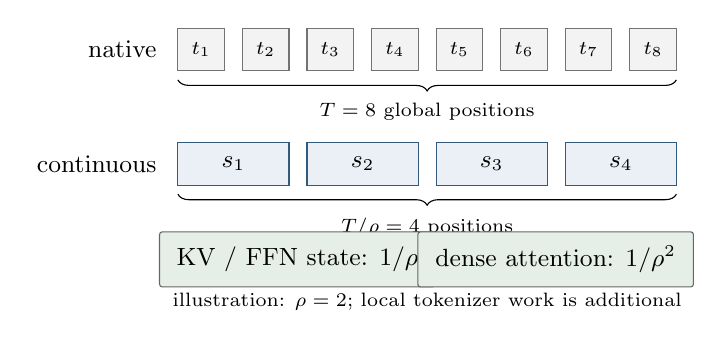
\begin{tikzpicture}[font=\small, x=0.82cm, y=0.82cm]
  \node[anchor=east] at (-0.18,1.35) {native};
  \foreach \x in {0,...,7} {
    \draw[fill=grayfill, draw=black!55] (\x,1.02) rectangle +(0.72,0.66);
    \node[font=\scriptsize] at (\x+0.36,1.35) {$t_{\the\numexpr\x+1\relax}$};
  }
  \draw[decorate, decoration={brace, amplitude=4pt, mirror}]
    (0,0.88) -- (7.72,0.88) node[midway, below=5pt, font=\scriptsize] {$T=8$ global positions};

  \node[anchor=east] at (-0.18,-0.42) {continuous};
  \foreach \x in {0,2,4,6} {
    \draw[fill=accentlight, draw=accent] (\x,-0.75) rectangle +(1.72,0.66);
  }
  \node at (0.86,-0.42) {$s_1$};
  \node at (2.86,-0.42) {$s_2$};
  \node at (4.86,-0.42) {$s_3$};
  \node at (6.86,-0.42) {$s_4$};
  \draw[decorate, decoration={brace, amplitude=4pt, mirror}]
    (0,-0.89) -- (7.72,-0.89) node[midway, below=5pt, font=\scriptsize] {$T/\rho=4$ positions};

  \node[valid, minimum width=35mm, minimum height=7mm] at (1.85,-1.90)
    {KV / FFN state: $1/\rho$};
  \node[valid, minimum width=35mm, minimum height=7mm] at (5.85,-1.90)
    {dense attention: $1/\rho^2$};
  \node[font=\scriptsize] at (3.86,-2.55)
    {illustration: $\rho=2$; local tokenizer work is additional};
\end{tikzpicture}}
\caption{For identical source bytes, denser spans shorten the global sequence. KV and per-position
work scale linearly in position count; dense prefill attention has a quadratic sequence term.}
\label{fig:positionbars}
\end{subfigure}
\caption{Analytical sources of potential memory and compute savings. These diagrams show scaling
relationships, not measured end-to-end speedups.}
\label{fig:systems}
\end{figure*}

\section{Preliminary Observations}

Preliminary experiments exercised both directional paths, but do not yet validate the complete
architecture. An exploratory three-seed Qwen output-only study bypassed the native vocabulary head
and emitted more than one byte per macro-step. It did not learn exact next spans or faithful
rollouts (Table~\ref{tab:prototype}). These results establish feasibility of the directional
interface while locating the central unsolved optimization problem.

\begin{table}[t]
\centering
\caption{Exploratory output-only observations. These measurements are diagnostic and do not
constitute a supported combined-system result.}
\label{tab:prototype}
\small
\begin{tabularx}{\columnwidth}{@{}X r@{}}
\toprule
Measurement & Three-seed mean \\
\midrule
Native vocabulary head bypass & yes \\
Bytes per global macro-step & 10.96 \\
Valid non-empty termination & 99.79\% \\
Byte accuracy & 17.91\% \\
Exact next-span fraction & 0.0096\% \\
Rollout byte agreement & 5.19\% \\
Output codec / native-head state & 4.65\% \\
\bottomrule
\end{tabularx}
\end{table}

An earlier input efficiency pilot also selected no feasible candidate: its best normalized
embedding RMSE was $0.8995$ against a prospectively registered $0.01$ ceiling. That outcome does
not prove finite-table overfitting impossible; it shows that the tested architecture, capacity,
budget, and objective did not solve it. The next study must isolate approximation capacity from
reconstruction and density by first overfitting a fixed vocabulary subset, scaling capacity while
remaining below the removable matrix budget, and only then restoring the full objective.

The important distinction is between \emph{protocol verification} and \emph{empirical evidence}.
Controlled synthetic tests can establish exact fallback, exhaustive non-monotonic segmentation,
cache neutrality, and frozen-backbone wiring. Only completed real-model experiments can support
embedding compatibility, behavioral preservation, density, or measured savings.

\section{Evaluation Protocol}

The proposal should be accepted or rejected claim by claim, not by a single celebratory score.
All thresholds, revisions, seeds, and held-out sets should be fixed before final runs.

\paragraph{Input compatibility.}
Measure normalized RMSE, cosine distribution, full-table retrieval, source-dtype bit equality, and
exact byte reconstruction for every unambiguous ordinary native payload. Compare native and
compatibility paths on KL and Jensen-Shannon divergence, top-$k$ agreement, NLL, perplexity, and
greedy generation.

\paragraph{Input density.}
Measure exact round-trip, bytes per continuous position, native-to-continuous position ratio,
fallback rate, span-length histogram, and invalid candidates by length on held-out natural
language, multilingual text, code, UTF-8/16/32 fixtures, and arbitrary binary bytes. The headline
must require 100\% round-trip.

\paragraph{Output quality and density.}
Measure exact next-span and byte accuracy, proper termination, control accuracy, native-feedback
equivalence, bytes per macro-step, rollout edit similarity, likelihood, calibration, and sampling
diversity. Output density counts only exact emitted bytes.

\paragraph{Combined-system behavior.}
Close the continuous feedback loop and compare sequence likelihood and generation behavior against
the native model under identical prompts. Verify that no ordinary vocabulary tensor is loaded or
serialized. For tied models, this is the first configuration in which complete removal is
applicable.

\paragraph{Systems performance.}
In isolated processes, report serialized and resident state, peak memory, tokenizer preparation,
prefill, time to first byte, decode latency, KV bytes, and energy when available. Run
cache-disabled, cold-cache, and warm-cache conditions. Include all local-module computation and
cache memory.

\paragraph{Replication.}
Use at least three fixed seeds and two tokenizer families. Publish every failed trial and preserve
immutable manifests. A result may be operationally complete while scientifically unsupported.

\section{Limitations and Open Problems}

\paragraph{Predictability is not reconstructability.}
A codec may reconstruct a long random identifier from its observed bytes, while an output model
cannot predict that identifier from context in one macro-step. Span selection may ultimately need
a rate or surprise criterion in addition to local validity.

\paragraph{Continuous generation needs a probability model.}
Greedy region membership is enough for deterministic decoding, but high-quality sampling requires
calibrated probabilities over variable-length byte sequences. Parallel output positions are
efficient but may model intra-span dependence less naturally than an autoregressive local decoder.

\paragraph{Finite precision bounds capacity.}
A finite-width, finite-precision latent cannot injectively represent arbitrary unbounded byte
strings. Bounded spans and atomic fallback make the protocol total; they do not make compression
free.

\paragraph{Native aliases can be contradictory.}
If two ordinary vocabulary rows map to identical canonical bytes but have different embeddings, a
deterministic encoder cannot reproduce both. Compatibility claims must be restricted to a
canonical reachable mapping or preserve the distinction structurally.

\paragraph{Local overhead can dominate.}
The combined architecture removes large vocabulary interfaces but adds local attention, decoding,
verification, and segmentation. It is simpler in discrete semantics and asymptotic vocabulary
state, not automatically in latency or implementation complexity.

\paragraph{Frozen-model replacement is the hard setting.}
An existing backbone was trained around native boundaries. Exact row imitation is a strong bridge,
but merged spans still change position count and internal computation. A model trained from scratch
with continuous tokens may realize more of the idea's potential, yet would provide weaker evidence
that the method is a drop-in replacement.

\section{Research Outlook}

Continuous tokens suggest a model whose vocabulary is procedural rather than enumerated. Frequent
spans may live in an ordinary memoization cache; rare or novel spans are composed by the same local
network. The cache accelerates the model without defining what it can represent. Languages,
encodings, code, and arbitrary binary streams share one protocol. New terms need no vocabulary
resize, and a fixed global context budget can represent more source bytes where the local codec is
effective.

The modular path makes the research tractable. Input-only experiments ask whether observed bytes
can replace fixed lookup and compress context. Output-only experiments ask whether hidden states
can predict exact byte spans and bypass a vocabulary head. The combined experiment asks whether
the two independently validated modules can close the loop and eliminate ordinary vocabulary state.
Each answer is useful, including a negative one.

\section{Conclusion}

The Transformer does not intrinsically require token IDs; it requires a sequence of vectors and a
well-defined output distribution. Continuous byte-span tokenizers move discrete structure to the
smallest universal boundary, retain exactness through local reconstruction, and allow the global
sequence to become denser. Their strongest form replaces both ordinary vocabulary matrices with
small directional byte modules around the backbone. Their most practical strength is modularity:
input-only and output-only adoption are independently meaningful, while composition unlocks the
full vocabulary-free architecture.

The proposal remains ambitious. Preliminary experiments establish execution paths and expose the
hard problems, not the final scientific result. That is precisely why the idea is valuable as a
research program: its claims are concrete, its failure modes are visible, and its potential benefits span
model state, context length, KV cache, global compute, multilinguality, and architectural clarity.

{\small
\bibliographystyle{plainnat}
\bibliography{references}
}

\end{document}
